\ifSTANDALONE
\section{Fallback}
\fi
\ifEMBED
\subsubsection{Fallback}
\fi
Ist der Einsatz des vorgesehenen BLDC-Treibers nicht möglich, so muss eine
alternative Ansteuerung erfolgen. Eine solche kann mit einer handelsüblichen
Steuerungen aus dem Modellbau erfolgen. Eine solche BLDC-Steuerung ist per
PWM angesteuert, wobei die im Modellbau üblichen Signale gelten, wie in der
Abbildung \ref{fig:rc-pwm} dargestellt.

\begin{figure}[h!]
	\centering
	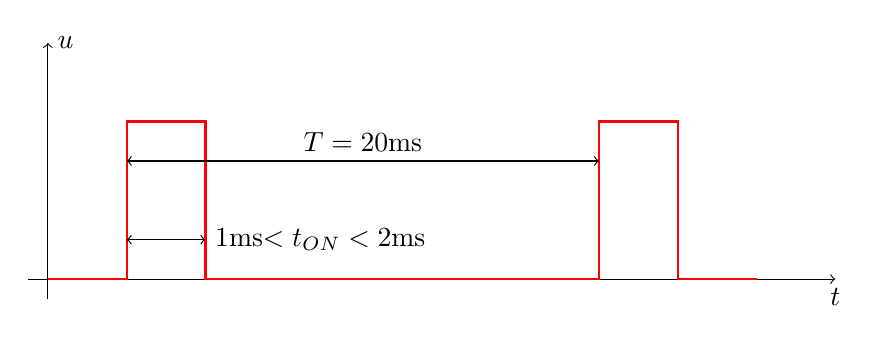
\begin{tikzpicture}
		% Achsen
		\draw[->] (-0.25,0) -- (10,0) node[anchor=north] {$t$};
		\draw[->] (0,-0.25) -- (0,3) node[anchor=west] {$u$};
		% Signal
		\draw[-,red,thick] (0,0) -- (1,0) -- (1,2) -- (2,2) -- 
			(2,0) -- (7,0) -- (7,2) -- (8,2) -- (8,0) -- (9,0);
		% Zeiten
		\draw[<->] (1,1.5) -- (7,1.5) node[midway, above] {$T=20$ms};
		\draw[<->] (1,0.5) -- (2,0.5) node[right] {$1$ms$<t_{ON}<2$ms};
	\end{tikzpicture}
	\caption{Signalverlauf eines typischen Modellbau-PWM Signals}
	\label{fig:rc-pwm}
\end{figure}

Der Einsatz von Modellbausteuerungen für BLDC-Motoren erfordert ein
Feedback der Drehzahl, da diese lediglich eine Steuerung darstellen. Die
Drehzahlregelung muss über eine externe Einheit erfolgen, beispielsweise einen
Mikrocontroller. Solche BLDC-Steuerungen werden im Modellbau typischerweise als
\emph{Regler} vertrieben und sind auch für hohe Leistungen durchaus preiswert.

\ifSTANDALONE
\subsection{Konzeptbeschreibung}
\fi
\ifEMBED
\newpage
\paragraph{Konzeptbeschreibung}$~~$\vspace{2mm}\\
\fi
Um eine Regelung der Drehzahl des BLDC-Motors zu ermöglichen, bedarf es eines
Feebacks, welches die Drehzahl wiedergibt. Dies ist mit einem
Hall-Effekt-Schalter zu realisieren. Dieser reagiert auf die Magnetfelder,
welche durch Magnete auf dem Rotationskörper gegeben sind. Aus solch einem
Aufbau resultiert ein Feedback, welches mit Impulsen einen Segmentdurchlauf
des Rotationskörpers wiedergibt, wie in Abbildung \ref{fig:fallback-sketch}
dargestellt.
\begin{figure}[h!]
	\centering
	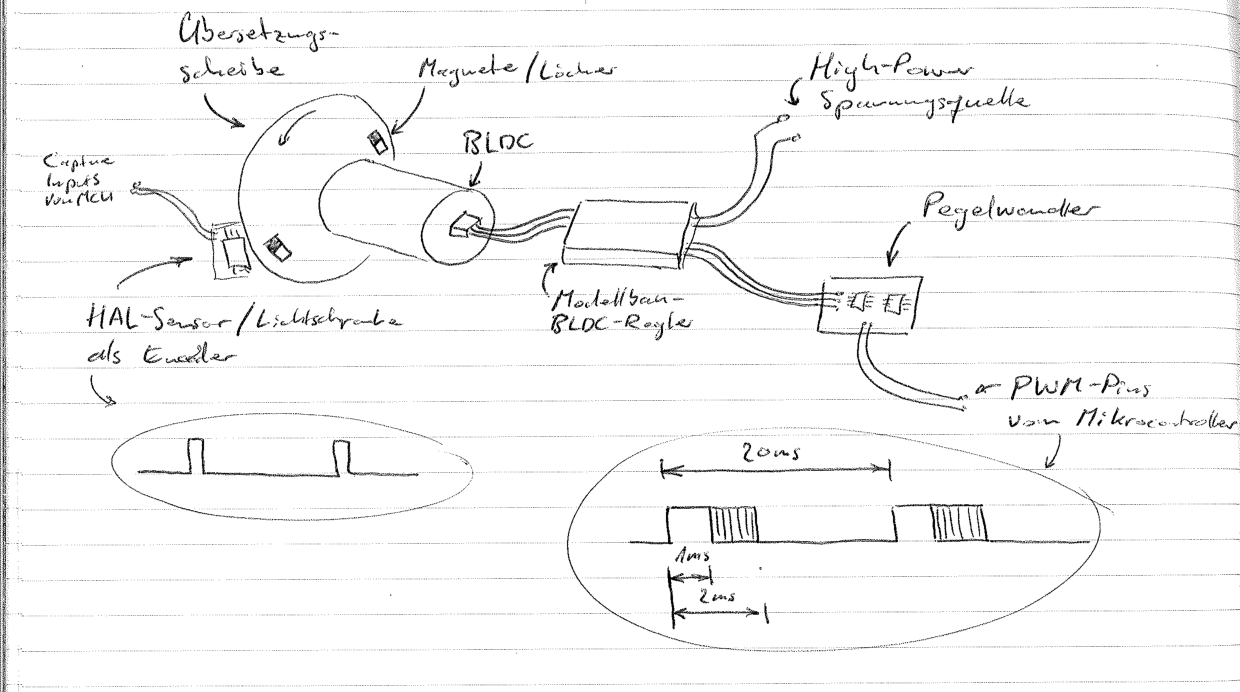
\includegraphics[width=0.8\textwidth]{\EtPath/Bilder/fallback_sketch_1.pdf}
	\caption{Erste Skizze des Fallback-Konzepts}
	\label{fig:fallback-sketch}
\end{figure}
Dieses Feedback wird mittels eines Mikrocontrollers ausgewertet und regelt
damit den Input der Steuerung mit dem PWM-Signal beziehungsweise der Impulsdauer.
Das Einlesen einer Flanke, die Zeitmessung bis zur nächsten Flanke und die
Stellung eines PWM-Signals, sind Tasks welche übliche Mikrocontroller direkt
durch ihre Peripherie-Module ausführen können. Dies ermöglicht eine einfache
Adaption in ein bestehendes Modell, denn es werden lediglich zwei Timer-IO
für diesen Fallback verwendet. Je nach Mikrocontroller ist ein Pegelwandler
für die PWM-Signale notwendig.
